\documentclass[12pt, titlepage]{article}

\usepackage{graphicx}
\usepackage{booktabs}
\usepackage{amssymb}
\usepackage{xr}
\externaldocument[ext1-]{../../SRS/CA}
\externaldocument[ext2-]{../../Design/MG/MG}
\externaldocument[ext3-]{../../Design/MIS/MIS}
\externaldocument[ext4-]{../../VnVPlan/SystVnVPlan/SystVnVPlan}
\externaldocument[ext5-]{../../UserGuide/UserGuide}
\externaldocument[ext6-]{../../VnVPlan/UnitVnVPlan/UnitVnVPlan}
\usepackage{tabularx}
\usepackage{hyperref}
\hypersetup{
    colorlinks,
    citecolor=black,
    filecolor=black,
    linkcolor=red,
    urlcolor=blue
}
\usepackage[round]{natbib}
\newcommand{\myprogname}{Lattice Boltzmann Solver} 
%% Comments

\usepackage{color}

\newif\ifcomments\commentstrue

\ifcomments
\newcommand{\authornote}[3]{\textcolor{#1}{[#3 ---#2]}}
\newcommand{\todo}[1]{\textcolor{red}{[TODO: #1]}}
\else
\newcommand{\authornote}[3]{}
\newcommand{\todo}[1]{}
\fi

\newcommand{\wss}[1]{\authornote{blue}{SS}{#1}} 
\newcommand{\plt}[1]{\authornote{magenta}{TPLT}{#1}} %For explanation of the template
\newcommand{\an}[1]{\authornote{cyan}{Author}{#1}}


\begin{document}

\title{Unit Test Report: \myprogname} 
\author{Peter Michalski}
\date{\today}
	
\maketitle

\pagenumbering{roman}

\section{Revision History}

\begin{tabularx}{\textwidth}{p{3cm}p{2cm}X}
\toprule {\bf Date} & {\bf Version} & {\bf Notes}\\
\midrule
Dec. 15 & 1.0 & Initial Document\\
\bottomrule
\end{tabularx}

~\newpage

\section{Symbols, Abbreviations and Acronyms}

Please see Section \ref{ext1-CASYMBOLS} and Section \ref{ext1-CAABBACR} of the Commonality Analysis (\citet{LBM_CA_PM}).

\newpage

\tableofcontents

\listoftables %if appropriate

\listoffigures %if appropriate

\newpage

\pagenumbering{arabic}

This document reports the results of the tests found in the Unit VnV Plan (\citet{LBM_UVNV_PM}).

\section{Functional Requirements Evaluation}

Functional requirements are evaluated in unit tests of id1 to id10. The results of these tests can be found in Section \ref{unittesting}. Traceability of the tests of this document to functional requirements is found in Table \ref{Table:TRCFR} of Section \ref{traceabilitytoreq}. 



\section{Nonfunctional Requirements Evaluation}

NFRs are evaluated in unit tests of id11 to id12. The results of these tests can be found directly below. Traceability of the tests of this document to NFRs is found in Table \ref{Table:TRCNFR} of Section \ref{traceabilitytoreq}.
		
\subsection{Performance}

Unit test id11 (performance-id11) found in Section \ref{ext6-M2performance} of the Unit VnV Plan (\citet{LBM_UVNV_PM} gathers information about the performance of the simulation section of M2SystemControl as the Reynolds Number input is increased.\\ 


\begin{figure}[h!]
	\begin{center}
		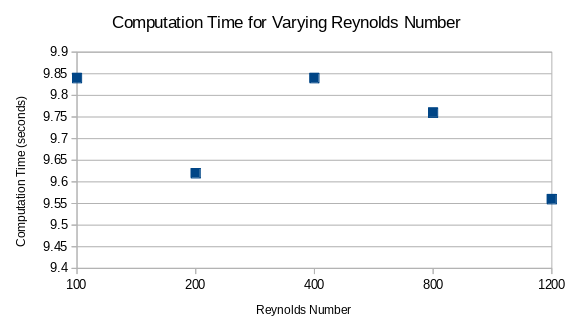
\includegraphics[width=1.0\textwidth]{compreynolds}
		\caption{Computation Time for Varying Reynolds Number}
		\label{Fig_ComputationTimeReynolds}
	\end{center}
\end{figure}

\noindent As we can see from Figure \ref{Fig_ComputationTimeReynolds} below, the computational time of the program is not affected as the Reynolds Number parameter is increased within the acceptable range.

~\newpage
\subsection{Scalability}
\label{nfrscalability}

Unit test id12 (scalability-id12) found in Section \ref{ext6-M9scalability} of the Unit VnV Plan (\citet{LBM_UVNV_PM} verifies if the M9Lattice module can be modified to return additional velocity weights of differing LBM parameters.\\

\noindent The system returned an output of: ``[0.6666666666666667, 0.1666666666666667, 0.1666666666666667]''. These values are the velocity weights for a problem that has 1 dimension and 3 velocity directions, verifying that M9Lattice is scalable for LBM problems of varying dimensions and velocity directions. 

\section{Comparison to Existing Implementation}	

The first stage of implementation will not incorporate the M9Lattice module since the library that will be used at this stage will incorporate the functions of that module in the M5LBMControl module. Thus, the test in Section \ref{nfrscalability} is not relative to the current stage of the system, but will be relevant in future development.

\section{Unit Testing}
\label{unittesting}

\subsection{M2SystemControl}
\subsubsection{problem-boundary-data-id1}
\label{M2id1}

Unit test id1 found in Section \ref{ext6-m2frtest} of the Unit VnV Plan (\citet{LBM_UVNV_PM} verifies if the M8Problem module and M10Boundary module return correct and correctly formatted parameters.\\

\noindent The md5sum hash value of the test file 'problem-boundary-data-id1.txt' is  0b332c9b4fc94adbb9c3f2e9a078fdb7. The hash value of the test output result is 5e518335d4054b401b83e699446a31c7.\\ 

\noindent Since the test resulted in a negative match a closer inspection of the two files was conducted and it was found that the returned data structure contains what appears to be a hashed value of either time or a location in the system that is used purely for identification purposes. The final output image of the system appears to be identical, however further testing may be required to conclusively confirm the hypothesis regarding the assumed identification hash found in the files. 

\subsubsection{simulation-id2}
\label{M2id2}

Unit test id2 found in Section \ref{ext6-m2frtest} of the Unit VnV Plan (\citet{LBM_UVNV_PM} verifies if the solution returned in the section of code representing M5LBMControl module is correct.\\

\noindent The md5sum hash value of the test file 'simulation-id2.txt' is\\  3e4fe44bbc9278d6536366a57ec8f467. The hash value of the test output result is 3e4fe44bbc9278d6536366a57ec8f467.\\ 

\noindent This confirms that the output of the section of code representing M5LBMControl module is correct. It also confirms the assumption in test id1 above that the differing hash value found within the test file 'problem-boundary-data-id1.txt' and the output of test id1 is not used in the actual simulation, as this test used the above section of code prior to calculating the LBM solution the output of which turned out to be identical between the control output and the test output. 

\subsection{M3InputReading}
\subsubsection{input-reading-id3}

Unit test id3 found in Section \ref{ext6-inreading} of the Unit VnV Plan (\citet{LBM_UVNV_PM} verifies if the module correctly handles not being able to find an input file.\\

\noindent Output of test: An error message of ``Input file not found.'' was printed to log\_file.log.\\

\noindent This output confirms that the module handles missing parameters correctly. 

\subsection{M4InputChecking}
\subsubsection{known-input-variables-id4}

Unit test id4 found in Section \ref{ext6-inchecking} of the Unit VnV Plan (\citet{LBM_UVNV_PM} verifies if the system correctly identifies a situation where the user provided input keys of the input.txt file are known to the system.\\

\noindent Output of test: An message of ``All parameters known.''.\\

\noindent This output confirms that the module correctly identifies a situation where an input file has known keys.

\subsubsection{unknown-input-variables-id5}

Unit test id5 found in Section \ref{ext6-inchecking} of the Unit VnV Plan (\citet{LBM_UVNV_PM} verifies if the system correctly identifies a situation where the user provided input keys of the input.txt file are unknown to the system.\\

\noindent Output of test: An error message of ``The parameter FakeField is not known to the system. Please see the User Guide.''  was printed to log\_file.log.\\

\noindent This output confirms that the module correctly identifies a situation where an input file has unknown keys.

\subsubsection{missing-input-requirements-id6}

Unit test id6 found in Section \ref{ext6-inchecking} of the Unit VnV Plan (\citet{LBM_UVNV_PM} verifies if the system correctly identifies a situation where the selected Library and Problem do not have all required inputs present in the input.txt file.\\

\noindent Output of test: An error message of ``The input.txt file is missing (or has incorrect) required parameters for the designated problem. Please see the User Guide.'' was printed to log\_file.log.\\

\noindent This output confirms that the module correctly identifies a situation where an input file does not have all of the required inputs for a library problem.

\subsubsection{present-input-requirements-id7}

Unit test id7 found in Section \ref{ext6-inchecking} of the Unit VnV Plan (\citet{LBM_UVNV_PM} verifies if the system correctly identifies a situation where the selected Library and Problem do have all required inputs present in the input.txt file.\\

\noindent Output of test: A message of ``Required input variables present.''.\\

\noindent This output confirms that the module correctly identifies a situation where an input file does have all of the required inputs for a library problem.

\subsection{M8Problem}
\subsubsection{problem-output-id8}

Unit test id8 found in Section \ref{ext6-m8problemmoduletest} of the Unit VnV Plan (\citet{LBM_UVNV_PM} verifies if the generated output of the module is correctly formatted.\\

\noindent The md5sum hash value of the test file 'problem-output-id8.txt' is\\  28984d413764f684243ba3632da3ef3d. The hash value of the test output result is e9946e61dfb8ecf717fa082c109edcc8.\\ 

\noindent Since the test resulted in a negative match a closer inspection of the two files was conducted and it was found, just as in test id1 of Section \ref{M2id1}, that the returned data structure contains what appears to be a hashed value of either time or a location in the system that is used purely for identification purposes. The final output image of the system again appears to be identical. As found in test id2 of Section \ref{M2id2}, this one alphanumeric value is not relevant to the final correctness of the system.

\subsection{M9Lattice}
\subsubsection{lattice-return-id9}

Unit test id9 found in Section \ref{ext6-M9lattice} of the Unit VnV Plan (\citet{LBM_UVNV_PM} verifies if the module returns the correct velocity weights for an LBM problem.\\

\noindent Output of test: ``[0.4444444444444444, 0.1111111111111111,
\\0.1111111111111111, 0.1111111111111111, 0.1111111111111111,
\\0.027777777777777776, 0.027777777777777776, 0.027777777777777776,
\\0.027777777777777776]''\\

\noindent This output confirms that the module returns correct velocity weights for a specified problem.

\subsection{M10Boundary}
\subsubsection{boundary-return-id10}

Unit test id10 found in Section \ref{ext6-M10Boundary} of the Unit VnV Plan (\citet{LBM_UVNV_PM} verifies if the module returns desired boundary dimensions.\\

\noindent Output of test: ``\{’x\_min’: 0.0, ’x\_max’: 3.0, ’y\_min’: 0.0, ’y\_max’: 1.0\}''\\

\noindent This output confirms that the module returns the desired boundary dimensions.

\section{Changes Due to Testing}
No changes are necessary to the first stage of implementation due to these test results.

\section{Automated Testing}

The Unit VnV Plan (\citet{LBM_UVNV_PM}) specifies which unit tests were to be automated. Time constraints have resulted in manual testing of the tests reported in this document; however they will be automated in January 2020.

\section{Trace to Requirements}
\label{traceabilitytoreq}

A complete description of functional requirements is found in Section \ref{ext1-CAFRS} of the CA (\citet{LBM_CA_PM}).

\begin{table}[!h]
	\begin{center}
		\begin{tabular}{| c | c | c | c | c | c | c | c |}
			\hline
			& R1 & R2 & R3 & R4 & R5 & R6 & R7\\
			\hline
			id1 & \checkmark &\checkmark & \checkmark& \checkmark& \checkmark& &\\
			\hline
			id2 & \checkmark &\checkmark & \checkmark& \checkmark& \checkmark& \checkmark&\\
			\hline
			id3 & \checkmark & & & & & & \\
			\hline
			id4 & \checkmark &\checkmark &\checkmark & & & & \\
			\hline
			id5 & \checkmark &\checkmark &\checkmark & & & & \\
			\hline
			id6 & \checkmark &\checkmark &\checkmark & & & & \\
			\hline
			id7 & \checkmark & & \checkmark& & & & \\
			\hline
			id8 & \checkmark &\checkmark & \checkmark& \checkmark & \checkmark& & \\
			\hline
			id9 & & \checkmark& & \checkmark& \checkmark& & \\
			\hline
			id10 & \checkmark & \checkmark& \checkmark& \checkmark& & & \\
			\hline
			id11 & \checkmark & \checkmark& \checkmark&\checkmark & \checkmark& \checkmark& \\
			\hline
			id12 & & \checkmark & & \checkmark& \checkmark& & \\
			\hline
		\end{tabular}
		\caption{Traceability Matrix Showing the Connections Between Test Cases and Functional Requirements}
		\label{Table:TRCFR}
	\end{center}
\end{table}   

~\newpage

A complete description of NFRs is found in Section \ref{ext1-CANFRS} of the CA (\citet{LBM_CA_PM}).

\begin{table}[!h]
	\begin{center}
		\begin{tabular}{| c | c | c | c | c | c | c | c | c | c | c |}
			\hline
			Cases / NFR & 1 & 2 & 3 & 4 & 5 & 6 & 7 & 8 & 9 & 10\\
			\hline
			id1 & & & & & & & & & &\\
			\hline
			id2 & \checkmark& & & & & & & & &\\
			\hline
			id3 & & & & & & & & & &\\
			\hline
			id4 & & & & & & & & & &\\
			\hline
			id5 & & & & & & & & & &\\
			\hline
			id6 & & & & & & & & & &\\
			\hline
			id7 & & & & & & & & & &\\
			\hline
			id8 & \checkmark& & & & & & & & &\\
			\hline
			id9 & & & & & & & & & &\\
			\hline
			id10 & & & & & & & & & &\\
			\hline
			id11 & & & \checkmark& & & & & & &\\
			\hline
			id12 & & & & & & & & \checkmark& &\\
			\hline
		\end{tabular}
		\caption{Traceability Matrix Showing the Connections Between Test Cases and NFRs}
		\label{Table:TRCNFR}
	\end{center}
\end{table}  


\newpage
		
\section{Trace to Modules}	
\label{modulecoverage}	

A complete description of modules is found in the MG (\citet{LBM_MG_PM}). A traceability of unit tests to modules can be found in Table \ref{ext6-Table:MODCOVT} in Section \ref{ext6-tracemod} of the Unit VnV Plan (\citet{LBM_UVNV_PM}).

\section{Code Coverage Metrics}

Module coverage is guaranteed for those modules that are implemented and not outsourced to external libraries. Module coverage is outline in Table \ref{ext6-Table:MODCOVT} in Section \ref{ext6-tracemod} of the Unit VnV Plan (\citet{LBM_UVNV_PM}).

~\newpage

\bibliographystyle {plainnat}
\bibliography {../../../refs/References}

\end{document}